\subsection{Wyprowadzenie}
Rozważmy sobie rozkład na \(\real^2\) o następujących własnościach:
\begin{itemize}
	\item gęstość wokół każdego punktu zależy jedynie od odległości od środka układu (w szczególności rotacja nie zmienia rozkładu).
	\item wartości współrzędnych \(x\) i \(y\) są od siebie niezależne.
	\item ten rozkład jest ciągły.
\end{itemize}

Okazuje się, że istnieje tylko jeden taki rozkład (z dokładnością do stałej), nazywamy go standardowym rozkładem normalnym. Oznaczamy go przez \( Z \sim N(0,1) \).

Zgodnie z definicją, gęstość zależy jedynie od odległości punktu od środka układu współrzędnych. Możemy więc to zapisać jako:
    \[
    f((x, y)) = f(r) = f\pars{\sqrt{x^2 + y^2}} = g(x)h(y) = g(x)g(y)
    \]
Ostatnie przekształcenie wynika z tego, że nasza gęstość nie zależy od rotacji, więc możemy obrócić wszystko o \(90\) stopni.
Dodatkowo, dla punktu \((r, 0 )\) równanie przyjmie postać:
    \[
    f((r, 0)) = g(r)g(0)
    \]
gdzie \( g(0) \) jest stałą. Z tego powodu możemy wstępnie założyć, że \( f = g \) a potem całość odpowiednio przeskalować. Tak więc teraz mamy:
    \[
    f\pars{\sqrt{x^2 + y^2}} = f(x)f(y)
    \]
Niech:
    \[ 
    h(x) = f\pars{\sqrt{x}} 
    \]
Wtedy:
    \[ h(x^2) = f(x) \]
    \[ h(x^2 + y^2) = h(x^2)h(y^2) \]
    \[ h(x + y) = h(x)h(y) \]

Z ostatniego punktu można przez indkucję pokazać, że \( \forall_{n \in \natural} \forall_{x_1, \ldots, x_n \in \real} h(x_1 + \ldots + x_n) = h(x_1)\ldots h(x_n) \)
Niech \( h(1) = b \). Korzystając z poprzedniego faktu mamy, że \(\forall_{n \in \natural} h(n) = b^n \).

Teraz chcemy udowodnić to samo dla liczb wymiernych:
    \[
    h\pars{\frac{p}{q} + \ldots + \frac{p}{q}} = h(p) = b^p = h\pars{\frac{p}{q}}^q
    \]
Gdzie na początku mamy dokładnie \(q\) ułamków \( \frac{p}{q} \) w funkcji \(h\).
Przekształcając ostatnią równość otrzymujemy:
    \[
    h\pars{\frac{p}{q}} = b^{\frac{p}{q}}
    \]

Na koniec chcemy udowodnić to samo dla liczb rzeczywistych (co na wykładzie chyba pominęliśmy).
Z MFI pamiętamy, że każdą liczbę rzeczywistą możemy przybliżyć jakimś ciągiem liczb wymiernych, a bardziej formalnie:
    \[
    \forall_{x \in \real} \exists_{q_n} x = \lim_{n \to \infty} q_n
    \]
Gdzie \( q_n \) jest jakimś ciągiem liczb wymiernym. Z połączenia tego faktu i założenia o ciągłości funkcji \(h\) otrzymamy:
    \[
    h(x) = h\pars{\lim_{n \to \infty} q_n} = \lim_{n \to \infty}h(q_n) = \lim_{n \to \infty} b^{q_n} = b^{\lim_{n \to \infty} q_n} = b^x
    \]

Ustalmy:
    \[
    	b = e^c \implies h(x) = e^{cx}
    \]

Teraz podstawiamy to do naszej funkcji gęstości, uwzględniamy skalowanie i otrzymujemy:
    \[
    f(z) = a \cdot e^{cx^2}
    \]
Gdzie \( c < 0 \). \\


Przyjmijmy \( c = -\frac{1}{2} \). Teraz chcemy znaleźć stałą \( a \). Oczywiście chcemy, żeby pole pod naszą funkcją wynosiło 1, więc wystarczy obliczyć odpowiednią całkę.
Całki:
    \[
    \int_{-\infty}^{\infty} e^{-\frac{z^2}{2}} \diff z 
    \]
nie jesteśmy w stanie ładnie rozwiązać, więc posłużymy się takim trikiem:
    \begin{align*}
    \int_{-\infty}^{\infty} e^{-\frac{z^2}{2}} \diff z \cdot \int_{-\infty}^{\infty} e^{-\frac{z^2}{2}} \diff z &= \int_{-\infty}^{\infty} \int_{-\infty}^{\infty} e^{-\frac{x^2 + y^2}{2}} \diff x \diff y \\
    &= \int_0^{2\pi} \int_0^{\infty} e^{-\frac{r^2}{2}} \cdot e \diff r \diff \theta \\
    &= \int_0^{2\pi} \int_0^{\infty} e^{-u} \diff u \diff \theta \\
    &= \int_0^{2\pi} 1 \diff \theta = 2\pi
    \end{align*}
Gdzie kolejno druga i trzecia równość to przejście na współrzędne biegunowe, oraz podstawienie \( u = \frac{r^2}{2} \) (dlatego przyjęliśmy akurat \( c = -\frac{1}{2} \) ).
Dalej mamy:
    \[
    \int_{-\infty}^{\infty} e^{-\frac{z^2}{2}} \diff z = \sqrt{2\pi} \implies a = \frac{1}{\sqrt{2\pi}}
    \]

\begin{minipage}[c]{0.5\linewidth}
	\[
		f(z) = \frac{1}{\sqrt{2\pi}} e^{-\frac{z^2}{2}}
	\]
\end{minipage}
\quad
\begin{minipage}[c]{0.4\linewidth}
	\centering
	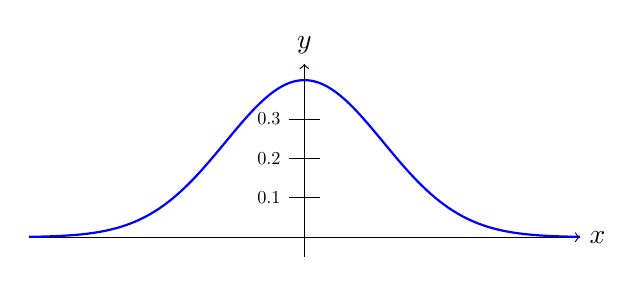
\begin{tikzpicture}
	\draw[->] (-3.5, 0) -- (3.5, 0) node[right] {$x$};
	\draw[->] (0, -0.25) -- (0, 2.2) node[above] {$y$};
	\draw[domain=-3.5:3.5, samples=100, yscale=5, smooth, variable=\x, blue, thick] plot ({\x}, {1/sqrt(2*pi) * exp(-0.5*\x*\x)});
	\draw (-0.2,0.5) -- (0.2,0.5);
	\node[scale=0.66] at (-0.45,0.5) {\(0.1\)};
	\draw (-0.2,1) -- (0.2,1);
	\node[scale=0.66] at (-0.45,1) {\(0.2\)};
	\draw (-0.2,1.5) -- (0.2,1.5);
	\node[scale=0.66] at (-0.45,1.5) {\(0.3\)};
\end{tikzpicture}
\end{minipage}

Funkcja gęstości prawdopodobieństwa standardowego rozkładu normalnego wygląda jak \sout{dzban} dzwon.


\subsection{Właściwości}
\begin{theorem}
	Wartość oczekiwana standardowego rozkładu normalnego wynosi 0, wariancja wynosi 1.
\end{theorem}

\begin{proof}
	Wartość oczekiwana wynosi 0, ponieważ standardowy rozkład normalny jest symetryczny wobec prostej \( OY\)
	Wariancja:
	\[
		\variance{Z} = \expected{Z^2} - \expected{Z}^2 = \expected{Z^2} = \\
	\]
	ponieważ \( \expected{Z} = 0 \)
	\[
		= \frac{1}{\sqrt{2\pi}}\int_{-\infty}^{z}t^2e^{-t^2/2} dt =
	\]
	\[
		= \frac{1}{\sqrt{2\pi}}\int_{-\infty}^{z}(t)(te^{-t^2/2}) dt =
	\]
	całkowanie przez części
	\[
		\brackets{-\frac{1}{\sqrt{2\pi}}te^{-t^2/2}}_{-\infty}^{\infty} + \frac{1}{\sqrt{2\pi}}\int_{-\infty}^{\infty}e^{-t^2/2} dt = 1
	\]
	Ponieważ pierwszy wyraz jest równy 0 a drugi jest to dystrybuanta na od \(-\infty \) do \( \infty \) więc wynosi ona 1.
\end{proof}
\begin{definition}
	Dystrybuantę standardowego rozkładu normalnego oznaczamy jako \( \Phi \), gdzie:
	\[
		\Phi(z) = \frac{1}{\sqrt{2\pi}} \int_{-\infty}^{z} e^{-\frac{t^2}{2}} \diff t
	\]
	Oraz:
	\[
		\Phi(-z) = 1 - \Phi(z)
	\]
	Ta całka generalnie nie jest do policzenia, jeżeli trzeba skorzystać z dystrybuanty to są do tego specjalne tabele wartości
\end{definition}
